% Options for packages loaded elsewhere
\PassOptionsToPackage{unicode}{hyperref}
\PassOptionsToPackage{hyphens}{url}
%
\documentclass[
  ignorenonframetext,
]{beamer}
\usepackage{pgfpages}
\setbeamertemplate{caption}[numbered]
\setbeamertemplate{caption label separator}{: }
\setbeamercolor{caption name}{fg=normal text.fg}
\beamertemplatenavigationsymbolsempty
% Prevent slide breaks in the middle of a paragraph
\widowpenalties 1 10000
\raggedbottom
\setbeamertemplate{part page}{
  \centering
  \begin{beamercolorbox}[sep=16pt,center]{part title}
    \usebeamerfont{part title}\insertpart\par
  \end{beamercolorbox}
}
\setbeamertemplate{section page}{
  \centering
  \begin{beamercolorbox}[sep=12pt,center]{part title}
    \usebeamerfont{section title}\insertsection\par
  \end{beamercolorbox}
}
\setbeamertemplate{subsection page}{
  \centering
  \begin{beamercolorbox}[sep=8pt,center]{part title}
    \usebeamerfont{subsection title}\insertsubsection\par
  \end{beamercolorbox}
}
\AtBeginPart{
  \frame{\partpage}
}
\AtBeginSection{
  \ifbibliography
  \else
    \frame{\sectionpage}
  \fi
}
\AtBeginSubsection{
  \frame{\subsectionpage}
}
\usepackage{amsmath,amssymb}
\usepackage{lmodern}
\usepackage{ifxetex,ifluatex}
\ifnum 0\ifxetex 1\fi\ifluatex 1\fi=0 % if pdftex
  \usepackage[T1]{fontenc}
  \usepackage[utf8]{inputenc}
  \usepackage{textcomp} % provide euro and other symbols
\else % if luatex or xetex
  \usepackage{unicode-math}
  \defaultfontfeatures{Scale=MatchLowercase}
  \defaultfontfeatures[\rmfamily]{Ligatures=TeX,Scale=1}
\fi
% Use upquote if available, for straight quotes in verbatim environments
\IfFileExists{upquote.sty}{\usepackage{upquote}}{}
\IfFileExists{microtype.sty}{% use microtype if available
  \usepackage[]{microtype}
  \UseMicrotypeSet[protrusion]{basicmath} % disable protrusion for tt fonts
}{}
\makeatletter
\@ifundefined{KOMAClassName}{% if non-KOMA class
  \IfFileExists{parskip.sty}{%
    \usepackage{parskip}
  }{% else
    \setlength{\parindent}{0pt}
    \setlength{\parskip}{6pt plus 2pt minus 1pt}}
}{% if KOMA class
  \KOMAoptions{parskip=half}}
\makeatother
\usepackage{xcolor}
\IfFileExists{xurl.sty}{\usepackage{xurl}}{} % add URL line breaks if available
\IfFileExists{bookmark.sty}{\usepackage{bookmark}}{\usepackage{hyperref}}
\hypersetup{
  pdftitle={A gentle introduction to the Variational Neural Networks},
  pdfauthor={J. Aubert and S. Donnet for StateOfTheR},
  hidelinks,
  pdfcreator={LaTeX via pandoc}}
\urlstyle{same} % disable monospaced font for URLs
\newif\ifbibliography
\usepackage{longtable,booktabs,array}
\usepackage{calc} % for calculating minipage widths
\usepackage{caption}
% Make caption package work with longtable
\makeatletter
\def\fnum@table{\tablename~\thetable}
\makeatother
\setlength{\emergencystretch}{3em} % prevent overfull lines
\providecommand{\tightlist}{%
  \setlength{\itemsep}{0pt}\setlength{\parskip}{0pt}}
\setcounter{secnumdepth}{-\maxdimen} % remove section numbering
\ifluatex
  \usepackage{selnolig}  % disable illegal ligatures
\fi

\title{A gentle introduction to the Variational Neural Networks}
\author{J. Aubert and S. Donnet for StateOfTheR}
\date{Dec.~2021}

\begin{document}
\frame{\titlepage}

\begin{frame}{Context}
\protect\hypertarget{context}{}
\begin{itemize}
\item
  In statistical learning, two main tasks:

  \begin{itemize}
  \tightlist
  \item
    \textbf{Regression or classification}
  \item
    \textbf{Reduction of dimension}
  \end{itemize}
\item
  Neural networks are used to construct the regression function,
  classifier or encoder-decoder (\textbf{autoencoder}).
\item
  \textbf{Variational versions} are used when we do not want to optimize
  a parameter but a \textbf{probability distribution}
\end{itemize}

\begin{longtable}[]{@{}
  >{\raggedright\arraybackslash}p{(\columnwidth - 0\tabcolsep) * \real{0.06}}@{}}
\toprule
\endhead
\# Organisation of the talk \\
- Relies on \\
1. \textbf{Regression and classification, reduction of dimension} \\
2. \textbf{Neural networks} \\
3. \textbf{Variational neural networks} \\
4. \textbf{A few reminder on the optimization procedure} \\
\bottomrule
\end{longtable}

class: center, middle

\begin{enumerate}
\tightlist
\item
  \textbf{Regression and classification, reduction of dimension}
\end{enumerate}
\end{frame}

\begin{frame}{Regression or classification}
\protect\hypertarget{regression-or-classification}{}
\begin{itemize}
\item
  Let \((\mathbf{X},\mathbf{Y})\) be our dataset:
\item
  \((\mathbf{X},\mathbf{Y})=(X_i, Y_i)_{i \in 1, \dots,N_{obs}}\)
\item
  \(\forall i =1,\dots,N_{obs}\), \textbf{Variables}
  \(X_i \in \mathbb{R}^n\).\\
\item
  \(Y_i \in \mathcal{Y}\) the variable to explain :
  \textbf{classification} or \textbf{regression}
\item
  Looking for a function \(f\)

  \begin{itemize}
  \item
    \textbf{classifier} or \textbf{regression}
    \(f :\mathbb{R}^n \mapsto \mathcal{Y}\) and
  \item
    such that
    \[Y \approx f(X) \Leftrightarrow \mbox{Loss}(Y -   f(X)) \mbox{ small } \]

    \begin{itemize}
    \item
      If \textbf{regression}
      \(\mbox{Loss}(Y - f(X)) = ||Y - f(X)) ||^2\)
    \item ~
      \hypertarget{if-classification-loss-cross-entropy}{%
      \subsection{\texorpdfstring{If \textbf{classification} : Loss =
      cross-entropy}{If classification : Loss = cross-entropy}}\label{if-classification-loss-cross-entropy}}
    \end{itemize}
  \end{itemize}
\end{itemize}
\end{frame}

\begin{frame}{Regression or classification}
\protect\hypertarget{regression-or-classification-1}{}
\begin{figure}

{\centering 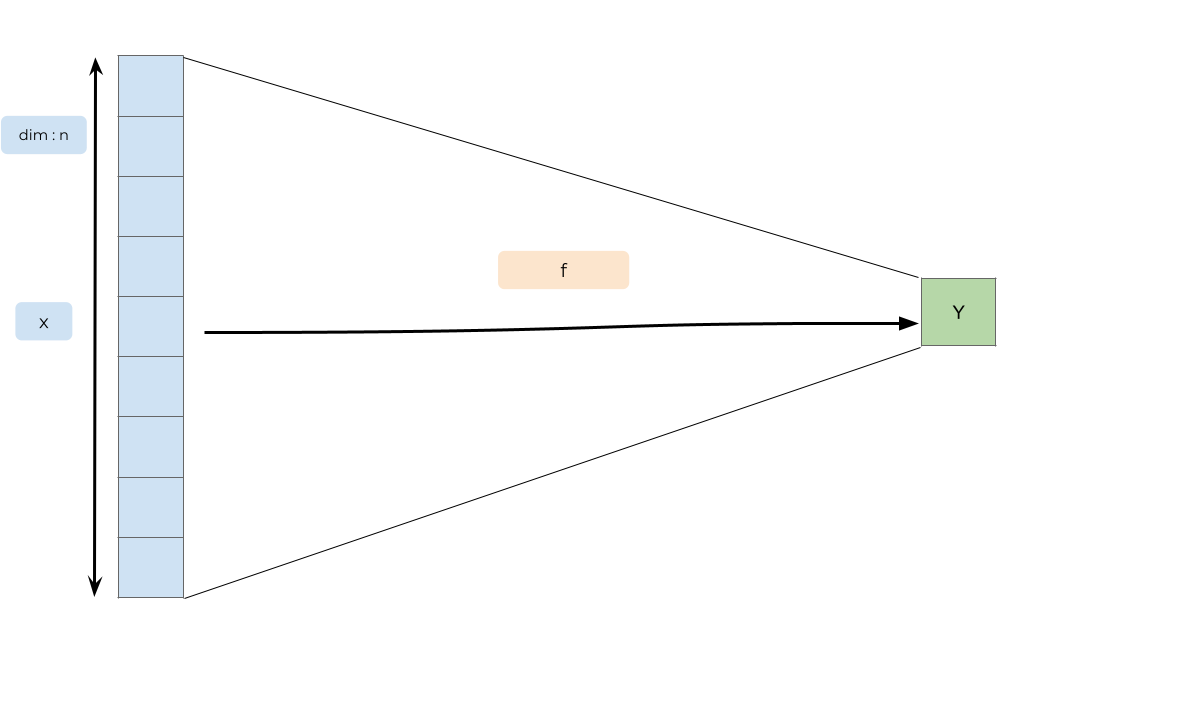
\includegraphics[width=0.9\linewidth]{images/RegressionClassification} 

}

\caption{Regression or classification}\label{fig:unnamed-chunk-1}
\end{figure}
\end{frame}

\begin{frame}{Reduction of dimension}
\protect\hypertarget{reduction-of-dimension}{}
\textbf{Auto-encoders} are used for the reduction of dimension of
(large) datasets.

- Let \(X\) be our dataset:
\(\mathbf{X}=(X_i)_{i \in 1, \dots,N_{obs}}\)

\begin{itemize}
\item
  \(\forall i =1,\dots,N_{obs}\), \(X_i \in \mathbb{R}^n\).
\item
  Looking for two functions

  \begin{itemize}
  \item
    \textbf{Encoder} \(e :\mathbb{R}^n \mapsto \mathbb{R}^m\) and
  \item
    \textbf{Decoder} \(d :\mathbb{R}^m \mapsto \mathbb{R}^n\)
  \item
    such that
    \[X \approx d(e(X)) \Leftrightarrow ||X -   d(e(X)) ||^2 \mbox{ small } \]
  \item
    \(Z = e(X)\) : \textbf{latent variable}
  \end{itemize}
\end{itemize}
\end{frame}

\begin{frame}{Autoencoder}
\protect\hypertarget{autoencoder}{}
\begin{figure}

{\centering 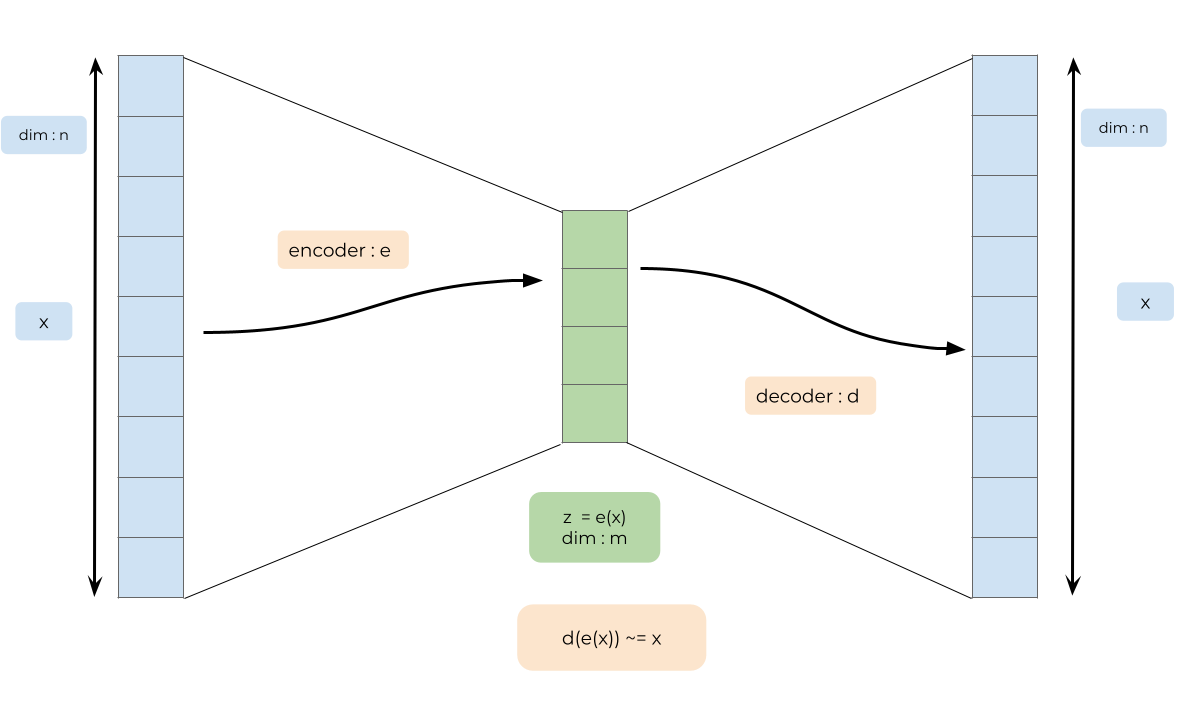
\includegraphics[width=0.9\linewidth]{images/Autoencoder} 

}

\caption{Autoencoder scheme.}\label{fig:unnamed-chunk-2}
\end{figure}

\begin{longtable}[]{@{}
  >{\raggedright\arraybackslash}p{(\columnwidth - 0\tabcolsep) * \real{0.06}}@{}}
\toprule
\endhead
class: middle \\
\textbf{Neural networks} \\
\bottomrule
\end{longtable}
\end{frame}

\begin{frame}{About \(f\): neural networks}
\protect\hypertarget{about-f-neural-networks}{}
\begin{figure}

{\centering 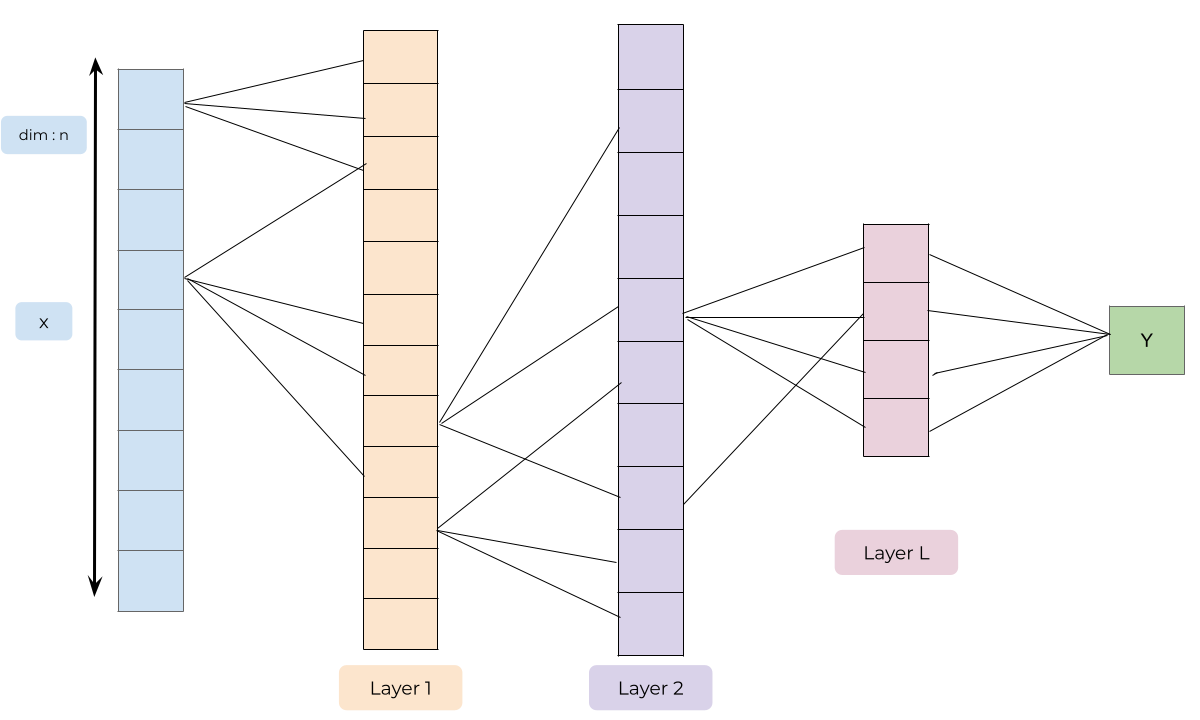
\includegraphics[width=0.9\linewidth]{images/NeuralNetwork} 

}

\caption{Neural network architecture.}\label{fig:unnamed-chunk-3}
\end{figure}
\end{frame}

\begin{frame}{About \(d\) and \(e\) : neural networks}
\protect\hypertarget{about-d-and-e-neural-networks}{}
\begin{figure}

{\centering 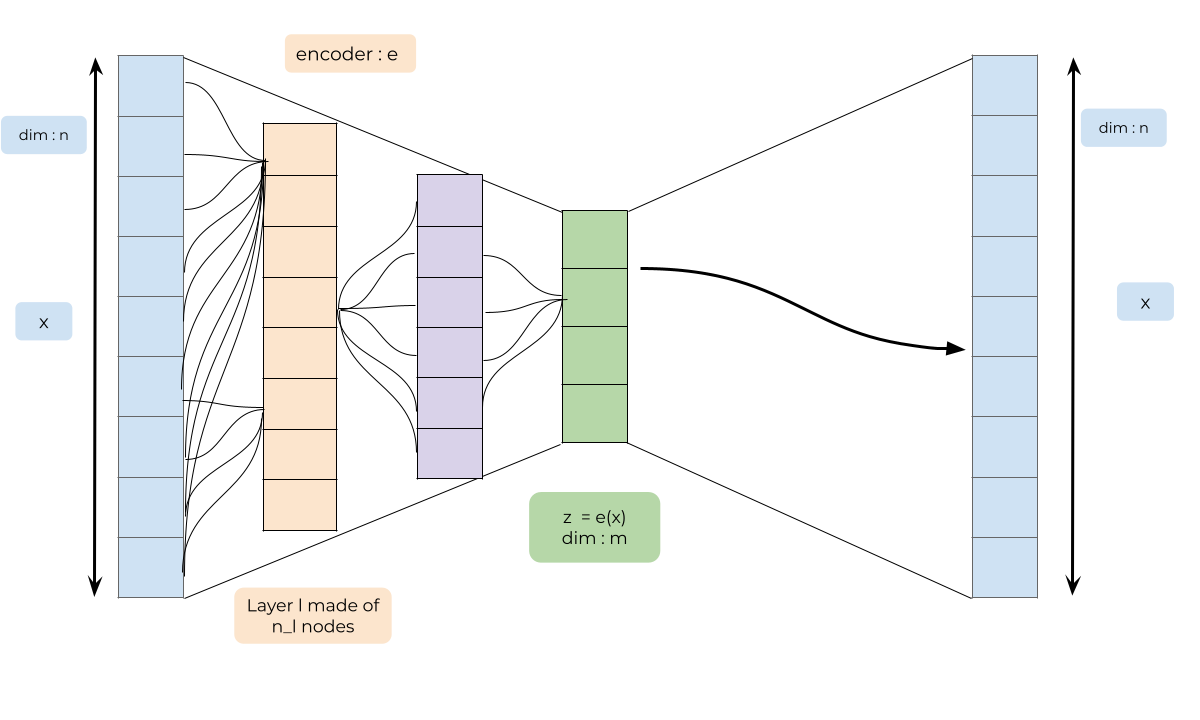
\includegraphics[width=0.9\linewidth]{images/Autoencoder2} 

}

\caption{Autoencoder scheme.}\label{fig:unnamed-chunk-4}
\end{figure}
\end{frame}

\begin{frame}{About neural networks}
\protect\hypertarget{about-neural-networks}{}
\textbf{One neuron} :
\(f_j (\mathbf{x}) = \phi (<w_j, \mathbf {x}> + \, b_j)\) where

\begin{itemize}
\item
  \(\phi\) the activation function : non linear
\item
  The quantities \(w_j = (w_j^1, \dots, w_j^n)\) are the weights of the
  input variables \((x^1, \dots, x^n)\)
\item
  \(b_j\) is the bias of neuron \(j\).
\end{itemize}

\textbf{At each layer} \(\ell\) of the neural network:

\begin{itemize}
\item
  Receive \(n_{\ell-1}\) input variables
  \(\mathbf{y}^{\ell-1} =(y^{\ell-1}_{1}, \dots,y^{\ell-1}_{n_{\ell-1}})\)
\item
  Create \(n_\ell\) new variables. For variable \(j\) of layer \(l\):
  \[y^{\ell}_{j} = \phi(<w^\ell_j, \mathbf{y}^{\ell-1}>  +  b^{\ell}_j)\]
\end{itemize}

\textbf{Unknown parameters} \(\theta\)\\
- \(w^\ell_j \in \mathbb{R}^{n_\ell-1}\), for \(\ell =1, \dots L\), for
\(j=1,\dots,n_{\ell}\), - \(b^\ell_j \in \mathbb{R}\), for
\(\ell =1, \dots L\), for \(j=1,\dots,n_{\ell}\),
\end{frame}

\begin{frame}{Model choice}
\protect\hypertarget{model-choice}{}
\textbf{To choose}:

\begin{itemize}
\item
  The number of layers \(L\)
\item
  The number of neurons in each layer: \(n_\ell\) :

  \begin{itemize}
  \tightlist
  \item
    possibly \(n_\ell > n\)
  \item
    For autoencoder the middle layer \(m < n\)
  \end{itemize}
\item
  The activation function \(\phi\)
\end{itemize}
\end{frame}

\begin{frame}{Learning \(f,d\) and \(e\)}
\protect\hypertarget{learning-fd-and-e}{}
\begin{itemize}
\tightlist
\item
  \textbf{Regression or classification}
\end{itemize}

The parameters
\(\theta = (w^\ell_j,b^\ell_j)_{j = 1\dots,n_\ell, \ell = 1,\dots,L}\)
are calibrated on a dataset \((X_i,Y_i)_{i=1, \dots , N_{obs}}\) by
minimizing the loss function

\[\widehat{\theta} = \mbox{argmin}_{\theta \in\Theta}  \sum_{i=1}^{N_{obs}}\mbox{Loss}(Y_i - f_{\theta}(X_i))\]

\begin{itemize}
\tightlist
\item
  \textbf{Autoencoder}
\end{itemize}

The parameters
\(\theta = (w^\ell_j,b^\ell_j)_{j = 1\dots,n_\ell, \ell = 1,\dots,L}\)
are calibrated on a dataset \((X_i)_{i=1, \dots , N_{obs}}\) by
minimizing the loss function

\[\widehat{\theta} = \mbox{argmin}_{\theta \in\Theta}  \sum_{i=1}^{N_{obs}}||X_i - d_{\theta}\circ e_{\theta}(X_i)||^2\]

\textbf{Optimisation by Stochastic gradient descent}: see later for a
reminder of the principle
\end{frame}

\begin{frame}{PCA versus autoencoder}
\protect\hypertarget{pca-versus-autoencoder}{}
\begin{itemize}
\item
  Let \(W \in M_{n,m}(\mathbb{R})\), \(W = (C_1,\dots,C_m)\)
\item
  The \(C_i\)'s are \(m\) columns vectors, \(m < n\).
\item
  \textbf{Hyp.}: \((C_i)\) are orthonormal vectors. Consequently:
  \[W'W = I_n\]
\item
  Let \(W' X_i\) is the projector of vector \(X_i\) on the sub-vectorial
  space generated by the columns of \(W\).
\item
  We are looking for \(W\) minimizing the inertia of the projected
  dataset: \[
  \begin{aligned}
  W^* &=\mbox{argmax}_{\{W \in M_{n,m}(\mathbb{R}), W'W = I_n\}} \sum_{i=1}^{N_{obs}} || W'X_i||^2\\ &=\mbox{argmin}_{\{W \in M_{n,m}(\mathbb{R}), W'W = I_n\}} \sum_{i=1}^{N_{obs}} || X_i - WW'X_i||^2
  \end{aligned}
  \]
\end{itemize}
\end{frame}

\begin{frame}[fragile]{PCA versus autoencoder}
\protect\hypertarget{pca-versus-autoencoder-1}{}
\begin{itemize}
\item
  \(W' = e\) \textbf{linear} encoder function
\item
  \(W = d\) : \textbf{linear} decoder function
\item
  Note that if you use neural networks with linear activation function
  and one layer, you will get \(W\) not necessarily orthogonal.
\end{itemize}

\href{http://www.xavierdupre.fr/app/mlstatpy/helpsphinx/c_ml/rn/rn_9_auto.html}{Lien
vers une démonstration propre}

\begin{longtable}[]{@{}
  >{\raggedright\arraybackslash}p{(\columnwidth - 0\tabcolsep) * \real{0.06}}@{}}
\toprule
\endhead
class: middle \\
\textbf{Variational versions} \\
\bottomrule
\end{longtable}

\begin{verbatim}
-   Prior on $\theta$: $\pi(\theta)$

-   Estimation not of $\theta$ but of the posterior distribution of $\theta$ : $p(\theta | \mathbf{Y})$
\end{verbatim}

\begin{itemize}
\item
  \textbf{Autoencoder}: give a structure on the latent space
  \(\mathbf{Z}\)

  \begin{itemize}
  \item
    Prior on \(Z\): \(\pi(Z)\)
  \item
    Estimation of \(\theta\) and of the posterior distribution of \(Z\)
    : \(p(Z | \theta, \mathbf{X})\)
  \end{itemize}
\item
  \textbf{Variational} : approximation of the distributions

  \begin{itemize}
  \item
    \(p(\theta | \mathbf{Y}) \approx q_\mathbf{Y}(\theta)\)
  \item
    \(p(Z | \theta, \mathbf{X}) \approx q_\mathbf{X}(Z)\)
  \end{itemize}
\end{itemize}
\end{frame}

\begin{frame}{Using the autoencoder to simulate}
\protect\hypertarget{using-the-autoencoder-to-simulate}{}
\begin{center}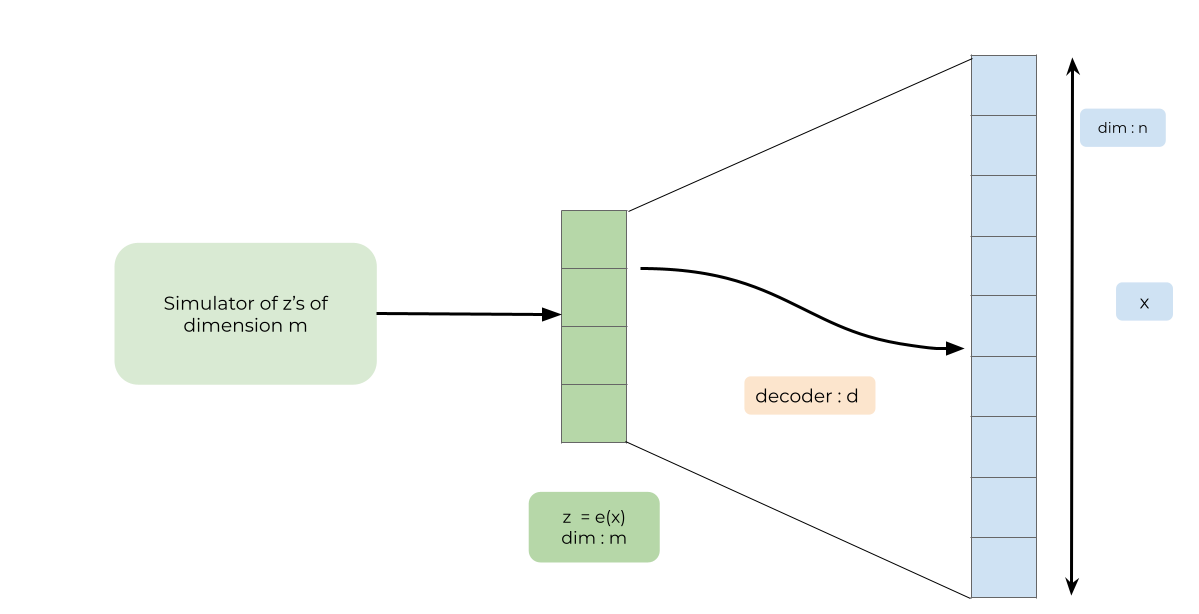
\includegraphics[width=0.7\linewidth]{images/VarAutoencoder} \end{center}

\begin{itemize}
\item
  The optimization of the autoencoder supplies
  \((Z_1, \dots, Z_{N_{obs}}) = (e(x_1), \dots, e(X_{N_{obs}}))\)
\item
  \textbf{How can we simulate the} \(z's\) such that \(d(z)\) looks like
  my original data?
\item
  How to construct a ``machine'' able to generate coherent other
  \(Z_i\).
\item
  Need to constrain/ structure the latent space.
\end{itemize}
\end{frame}

\begin{frame}{Probabilistic version of the autoencoder}
\protect\hypertarget{probabilistic-version-of-the-autoencoder}{}
\begin{itemize}
\item
  \textbf{Idea} : put a prior distribution on the latent space et
  estimate the posterior distribution.
\item
  \textbf{A statistical model with latent variables}
\end{itemize}

\[X_i =d(Z_i) + \epsilon_i\] \[Z_i \sim_{i.i.d.}N_m(0,I_m)\]
\[\epsilon_i \sim_{i.i.d.} \mathcal{N}_n(0,c I_n)\]

\begin{itemize}
\tightlist
\item
  Likelihood
  \[\ell(\mathbf{X}; d)  =  \int_{\mathbf{Z}} p(\mathbf{X} | \mathbf{Z};d)p(\mathbf{Z})d\mathbf{Z}\]
\end{itemize}
\end{frame}

\begin{frame}{Variational Bayesian inference}
\protect\hypertarget{variational-bayesian-inference}{}
\begin{itemize}
\tightlist
\item
  Approximate the posterior \(p(\theta | Y)\) by \(q(\theta)\) where
  \(q\in \mathcal{R}\)
\end{itemize}

\begin{itemize}
\item
  \textbf{Model} \(\ell(\mathbf{Y} | \theta)\)
\item
  \textbf{Prior} on \(\theta\) : \(\pi(\theta)\)
\item
  \textbf{Approximate the posterior} \(p(\theta | Y)\) by \(q(\theta)\)
  where \(q\in \mathcal{R}\) where \(\mathcal{R}\) family of simpler
  distributions

  \begin{itemize}
  \tightlist
  \item
    \textbf{Example}: \(q(\cdot) = \mathcal{N}(\mu,\Sigma)\)
  \end{itemize}
\end{itemize}

--

\begin{itemize}
\tightlist
\item
  Approximating = Minimizing the KL
\end{itemize}

\[\hat{q} = \arg\min_{q \in\mathcal{R}} D_\text{KL}(q(\theta),p(\theta | \mathbf{Y}))\]
where
\[ D_\text{KL}(q(\theta),p(\theta | \mathbf{Y})) = \mathbf{E}_q\left[\log \frac{q(\theta)}{p(\theta | \mathbf{Y})}\right]\]
\end{frame}

\begin{frame}{The magic trick}
\protect\hypertarget{the-magic-trick}{}
\[D_\text{KL}(q(\theta),p(\theta | \mathbf{Y}))  = \log \ell(\mathbf{Y}) - \left[\underbrace{\mathbf{E}_q[\log \ell(\mathbf{Y}|\theta)\pi(\theta)] -\mathbf{E}_q[\log q(\theta)]}_{\text{ELBO}}\right]\]

\begin{itemize}
\tightlist
\item
  \(\log \ell(\mathbf{Y})\) independent of \(q\)
\end{itemize}

\begin{itemize}
\tightlist
\item
  Minimizing the KL is equivalent to minimizing the Cost Function
\end{itemize}

\begin{eqnarray}
\mathcal{F}(q) &=& -  \mathbf{E}_q[\log \ell(\mathbf{Y}|\theta)\pi(\theta)] + \mathbf{E}_q[\log q(\theta)] \\
&=&  -  \mathbf{E}_q[\log \ell(\mathbf{Y}|\theta)] + \mathbf{E}_q\left[\log \frac{q(\theta)}{\pi(\theta)}\right] \\
&=&D_{\text{KL}}(q,\pi) -  \mathbf{E}_q[\log \ell(\mathbf{Y}|\theta)]   
\end{eqnarray}
\end{frame}

\begin{frame}
\#Parametrization of \(q\)

Choose a parametric form in \(q = q_{\eta}\). - \textbf{For example} :
\(q = \mathcal{N}(\mu,\Sigma)\)

\[\hat{\eta} = \arg\min_{\eta} \mathcal{F}(\eta) = \arg\min_{\eta} D_{\text{KL}}(q_{\eta},\pi) - \mathbf{E}_{q_{\eta}}[\log \ell(\mathbf{Y}|\theta)]\]

\begin{itemize}
\item
  Optimisation by gradient descent
\item
  \textbf{BUT} expectation not explicit
\end{itemize}
\end{frame}

\begin{frame}{Monte Carlo approximation}
\protect\hypertarget{monte-carlo-approximation}{}
\begin{itemize}
\item
  With neural networks,
  \(\mathbf{E}_{q_{\eta}}[\log \ell(\mathbf{Y}|\theta)]\) not explicit
  (activation functions non linear)
\item
  Approximation for Monte Carlo : assume that
  \(\theta^{(m)} \sim q_{\eta}\)
\end{itemize}

\[\widehat{\mathcal{F}}(\eta) = \frac{1}{M}\sum_{m=1}^M  \log q_{\eta}(\theta ^{(m)}) - \log \pi(\theta^{(m)}) -  \log \ell(\mathbf{Y}|\theta^{(m)})\]

\begin{itemize}
\item
  \textbf{Problem} we lost the explicit dependence in \(\eta\) through
  the simulations \(\theta^{(m)}\)
\item
  \textbf{Solution} : reparametrisation
  \(\xi\sim \mathcal{N}(0,\mathbf{I})\), and \(\phi = g(\xi,\eta)\)
\end{itemize}

\[\widehat{\mathcal{F}}(\eta) = \frac{1}{M}\sum_{m=1}^M   \log q_{\eta}(\phi(\xi^{(m)},\eta)) - \log \pi(\phi(\xi^{(m)},\eta)) - \log \ell(\mathbf{Y}| \phi(\xi^{(m)},\eta))\]
- \textbf{Remarks}

\begin{itemize}
\tightlist
\item
  \(M=1\)?
\item
  \(D_{\text{KL}}(q_{\eta},\pi)\) may be explicit (for Gaussian
  distributions for instance) but not used in practice
\item
  \(\xi^{(m)}\) are resimulated each time we compute the gradients
\end{itemize}
\end{frame}

\begin{frame}{More details for the regression case}
\protect\hypertarget{more-details-for-the-regression-case}{}
\begin{itemize}
\item
  \(\theta\) are the parameters (weights and bias)
\item
  Prior gaussian distribution on \(\theta\) :
  \(\theta \sim \mathcal{N}(0, \mathbb{I})\)
\item
  If regression
  \[Y_i = f_\theta(X_i) + \epsilon_i, \quad \epsilon \sim \mathcal{N}(0,\sigma^2)\]
\item
  \[\left[\sum_{i=1}^{N_{obs}}   \frac{||Y_i - f_{ \phi(\xi^{(m)},\eta) }(X_i)||^2}{2\sigma^2}\right]\]
\end{itemize}
\end{frame}

\begin{frame}{In the case of a neural network}
\protect\hypertarget{in-the-case-of-a-neural-network}{}
\begin{itemize}
\tightlist
\item
  \(\theta\) are the parameters (weights and bias)
\item
  Prior gaussian distribution on \(\theta\) :
  \(\theta \sim \mathcal{N}(0, \mathbb{I})\)
\item
  If regression
  \[Y_i = f_\theta(X_i) + \epsilon_i, \quad \epsilon \sim \mathcal{N}(0,\sigma^2)\]
\end{itemize}

\[\text{ELBO}(q) = \mathbb{E}_{q}  \left[\sum_{i=1}^{N_{obs}} - \frac{||X_i - f_{\theta}(X_i)||^2}{2\sigma^2}\right]\]
\end{frame}

\begin{frame}{Approximate the posterior distribution}
\protect\hypertarget{approximate-the-posterior-distribution}{}
\begin{itemize}
\item
  Since \(\ell(\mathbf{X}; d)\) is too difficult to tackle because of
  the form of \(p(\mathbf{Z} | \mathbf{X}; d)\)
\item
  Let's simplify that distribution
  \[p(\mathbf{Z}  | \mathbf{X};d) = \prod_{i=1}^{N} p(Z_i |  X_i; d)  \approx q_{\mathbf{X}}(\mathbf{Z};g,H)  = \prod_{i=1}^{N} q_{ X_i}(Z_i;g,H)\]
  \[q_{X_i}(Z_i;g,h) =\mathcal{N}_m(g(X_i),H(X_i))\]
\item
  Replace the likelihood by the ELBO
\end{itemize}

\[
\begin{eqnarray}
 ELBO(d,g,H) &=&\ell(\mathbf{X}; d)-  KL(q(\mathbf{Z};\mathbf{X},g,H), p\mathbf{Z} |\mathbf{X};d))\\
 &=&\mathbb{E}_{q_{\mathbf{X}}(\mathbf{Z}; ,g,H)}[\log p(\mathbf{X} , \mathbf{Z};d)] + Entr(q_{\mathbf{X}}(\mathbf{Z};g,H)))\\
 &=& \mathbb{E}_{q_{\mathbf{X}}(\mathbf{Z};g,H)}[\log p(\mathbf{X} | \mathbf{Z};d)]- KL(q_{\mathbf{X}}(\mathbf{Z};g,H), p(\mathbf{Z}))\\
\end{eqnarray}
 \]

\begin{longtable}[]{@{}
  >{\raggedright\arraybackslash}p{(\columnwidth - 0\tabcolsep) * \real{0.06}}@{}}
\toprule
\endhead
\# Maximize a variational lower bound
\((\hat{d},\hat{g},\hat{H}) = \mbox{argmin}_{d,g,H} ELBO(d,H,g)\) \\
\(ELBO(d,g,H)  = \mathbb{E}_{q_{\mathbf{X}}(\mathbf{Z};g,H)}[\log p(\mathbf{X} | \mathbf{Z};d)]- KL(q_{\mathbf{X}}(\mathbf{Z};g,h), p(\mathbf{Z}))\) \\
- \textbf{Reconstruction term} \\
\(\mathbb{E}_{q_{\mathbf{X}}(\mathbf{Z};g,H)}[\log p(\mathbf{X} | \mathbf{Z};d)] = \mathbb{E}_{q_{\mathbf{X}}(\mathbf{Z};g,H)}  \left[\sum_{i=1}^N - \frac{||X_i - f(Z_i)||^2}{2c}\right]\) \\
- \textbf{Regularisation term} : \(KL\) \\
- \(c\) : variance parameter which balances regularisation and
reconstruction \\
\bottomrule
\end{longtable}

\#About d

\(d\) neural network function as before
\end{frame}

\begin{frame}
\#About g and h

\begin{itemize}
\item
  Are called the ``encoder part''
\item
  \(g\) and \(H\):
\item
  \(H(X)\) is a covariance so

  \begin{itemize}
  \tightlist
  \item
    it should be a square symetric matrix
  \item
    \textbf{Simplification} : diagonal matrix \(H(X) = h'(X)h(X)\)
  \item
    \(h(X) \in \mathbb{R}^m\)
  \end{itemize}
\item
  \(h(X) = h_2(h_1(X))\), \(g(X) = g_2(g_1(X))\), \(g_1 = h_1\)
\end{itemize}

\begin{center}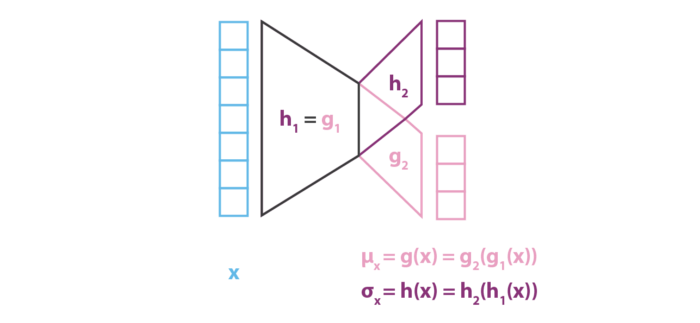
\includegraphics[width=0.9\linewidth]{images/approxZ} \end{center}
\end{frame}

\begin{frame}
\#Evaluation of the expectation

Note that the term
\(\mathbb{E}_{q_{\mathbf{X}}(\mathbf{Z};g,h)} \left[\sum_{i=1}^N - \frac{||X_i - f(Z_i)||^2}{2c}\right]\)
can not be evaluated.

So people simulate latent variable

\[\mathbb{E}_{q_{\mathbf{X}}(\mathbf{Z};g,h)}  \left[\sum_{i=1}^N - \frac{||X_i - f(Z_i)||^2}{2c}\right] \approx  \left[\sum_{i=1}^N - \frac{||X_i - f(g(X_i) + diag(h(X_i))\xi_i)||^2}{2c}\right]\]
where \(\xi_i\sim \mathcal{N}_m(0,\mathbb{I}_m)\)
\end{frame}

\end{document}
